\begin{figure}[]
    \centering
    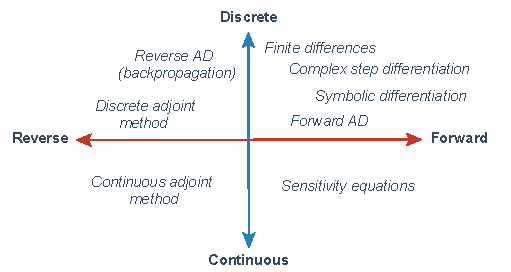
\includegraphics[width=0.80\textwidth]{figures/scheme-methods.pdf}
    \caption{Schematic representation of the different methods available for differentiation involving differential equation solutions. These can be classified depending if they find the gradient by solving a new system of differential equations (\textit{continuous}) or if instead they manipulate unit algebraic operations (\textit{discrete}). Furthermore, depending if these methods run in the same direction than the numerical solver, we are going to be talking about \textit{backward} and \textit{forward} methods.}
    \label{fig:diff}
\end{figure}
Depending on the number of parameters and the complexity of the differential equation we are trying to solve, there are different methods to compute gradients with different numerical and computational advantages and that also scale differently depending of the number of differential equations $n$ and number of parameters $p$.
These methods can be roughly classified as:
\begin{itemize}
    \item \textit{Discrete} vs \textit{continuous} methods.
    \item \textit{Forward} vs \textit{backwards} methods.
\end{itemize}
The first difference regards the fact that the method for computing the gradient can be either based on the manipulation of atomic operations that are easy to differentiate using the chain rule several times (discrete), in opposition to the approach of approximating the gradient as the numerical solution of a new set of differential equations (continuous).
Another way of conceptualizing this difference is by comparing them with the discretize-optimize and optimize-discretize approaches \cite{bradley2013pde, Onken_Ruthotto_2020}.   
We can either discretize the original system of ODEs in order to numerically solve it and then define the set of adjoint equations on top of the numerical scheme; or instead define the adjoint equation directly using the differential equation and then discretize both in order to solve \cite{Giles_Pierce_2000}.

The second distinction is related to the fact that some methods compute gradients by resolving a new sequential problem that may move in the same direction of the original numerical solver - i.e. moving forward in time - or, instead, they solve a new system that goes backwards in time. 
Figure \ref{fig:diff} displays a classification of some methods under this two-fold classification. In the following section we are going to explore more in detail these methods.

It is important to remark that all the 